\section{Deriving Transition Queries} 
In this section, we present our solution for efficiently generate transition queries. 

\subsection{Deriving Attribute Query Components} 

An attribute query has parameters: a pair of attributes or alignment, a source instance, a function of similarity and a threshold. In this work we assume that the function of similarity is given, as well as, its threshold.

\subsubsection{Pair of attributes or alignment}. As we described before, a list of attribute alignments between two sources can be obtained using state of the art schema alignment techniques. However, to our purpose, it only makes sense to select attributes that acts as denominator of an instance (e.g., title, label, name), which will call as \textit{relative identifiers}.Those attributes are very discriminative properties of the data and can be obtained by a simple but efficient entropy-based unsupervised method that we describe below.

\begin{definition}[Identifiers] An attribute $r_k$ is an identifier, if $\forall i,j, i \neq j$ $s_i(r_k) \neq  s_j(r_k)$. It means that all instances have a different value for this attribute.
\end{definition}  

\begin{definition}[Identifiers Distribution] Given $V_{rk}$ as the set of values of an identifier $r_k$,  the probability Pr[$v_i$]= 1/ $|V_{rk}| \forall v_i \in V_{rk}$ 
\end{definition}  

\begin{definition}[Relative Identifiers] Relative identifier are attributes where the distribution of their values is the closest to the distribution of an identifier.
\end{definition}  

As identifiers have a constant distribution, their entropy H($r_k$) is maximal and the ratio H($r_k$) / log($|V_{rk}| $)= 1. Using this property, we can now easily select attributes that are relative identifiers. For that, we only consider, from the alignment list produced by a schema alignment technique, the attributes pairs in which both attributes have an relative maximal entropy ratio. We exclude text and non-literal attributes(e.g., uris), which have high entropy ratio but are not good discriminative properties.   

The pseudo-code is described by the algorithm 1:

\begin{algorithm}
\caption{Select a list of relative identifier pairs}
\begin{algorithmic}
\STATE list = obtain attribute alignment between source and target datasets.
\STATE identifiers = $\emptyset$
\STATE max=0
\FORALL{(a,b) in list}
\STATE Ha = computes entropy ratio of the attribute a
\STATE Hb = computes entropy ratio of b
\IF{$(Ha > max$  and $Hb > max$) or (Ha is maximal or Hb is maximal)}
\STATE $identifiers \leftarrow  (a,b)$
\STATE max = ha
\ENDIF
\ENDFOR
\RETURN identifiers
\end{algorithmic}
\end{algorithm}
 
Then, we build an attribute query for each selected relative attribute pair. Notice that more than one pair may be selected. For instance, the pairs (label,title) and (phone, phonenumber). For those pairs, we would build the queries: $Q_a(s_i,label,title, \omega, \delta)$ and $Q_a( s_i, phone, phonenumber,  \omega, \delta)$. The attribute queries generated by this procedure are used as attribute query components of the transitions queries during the rest of the process. The only parameter that change from state to state in those queries is the instance $s_i$. Notice that future implementations of these framework may also vary the similarity function and threshold,  to better adapt to the characteristic of the attributes values. For instance, a specific similarity measure could be used for names, number, geographic information, etc.

\subsection{Deriving Class Query Components} 

\subsubsection{From a solution set to class queries}. Firstly, we are going to introduce an algorithm that given a set R of instances that are correct matches for a subset of instance in $S_C$, obtains a disjunction of class queries that selects those instances in R. Later, we will explain how we use this algorithm to generate class query components.  

Consider an instance representation as a set of attribute/value pairs, as well as, R as a set of those instances representations. By intersection all sets in R we could obtain the set of attribute/value pairs that occurs in all instances. However, this straightforward approach may also retrieve an empty set due to missing information on the data (e.g. no attribute occurs in all instances). To solve this issue, we elaborate another approach that uses the same principal of intersection of sets. The algorithm compares two instance representations; if they produce a non-empty set, then it joins both instances representations in one set. Otherwise, it keeps the instances as they were. It does this until all instances are compared. Then, for all resultant sets, it randomly extracts one attribute/value pair. Those pairs composes a disjunction of class queries. This algorithm is listed below:

\begin{algorithm}
\caption{Class Query Extractor Algorithm - Select class queries for a set of instances representations R}
\begin{algorithmic}
\STATE query = []
\FOR{$i = 0$ to $|R|-1$}
\FOR{$j = 1$ to $|R|$}
\STATE X = R[i] $\cap$ R[j]
\IF{X $\neq \emptyset$}
\STATE  R[i] =  X
\STATE  R[j]= $\emptyset$
\ENDIF
\ENDFOR
\ENDFOR 
\FOR{$i = 0$ to $|R|$}
\STATE query $\leftarrow$ select one pair from R[i]
\ENDFOR
\RETURN query
\end{algorithmic}
\end{algorithm}

In the worse case, this algorithm produces a class query with N clauses, where N is the size of R.  Its complexity is O($N^2$). However, notice that we apply this algorithm for a small set of instances, which does not impact the overall performance of the algorithm.

\subsubsection{Class Query Generation Flow}. We designed an incremental process to generate the class queries. Assuming that at specific intermediary state n we can find the correct matches for the candidate sets already produced at this state. Then, we can apply the previous algorithm \textit{class query extractor} to generate the class queries. The challenge is to solve the problem for the intermediary state n.  Generally, any refined approach for matching instances after blocking strategies could be used. In this work we used the class-based disambiguation implemented in SERIMI. The full process of generating the class queries from the candidate sets at a state n are depicted below:

\begin{figure} 
\centering
\includegraphics[width=\textwidth ]{p5.png}
\caption{The process of generating transition queries from the candidate sets} 
\end{figure} 

So far, we described both independent process of obtaining the attribute and class queries. The process of deriving the transition queries is  trivial. The transition queries are the cross-product between the attribute queries and class queries. For instance, given the set of attribute queries composed of the queries $Q_a(s_i,label,title, \omega, \delta)$ and $Q_a( s_i, phone, phonenumber,  \omega, \delta)$. And the set o class queries compose of the queries $Q_c(type, Movie)$ and $Q_c(type, Documentary)$. The 4 transitions queries for the settings would be: 
\\
\\
1) $Q_a(s_i,label,title, \omega, \delta) \wedge Q_c(type, Movie)$, \\
2) $Q_a( s_i, phone, phonenumber,  \omega, \delta) \wedge Q_c(type, Movie)$,  \\
3) $Q_a(s_i,label,title, \omega, \delta) \wedge Q_c(type, Documentary)$ and \\
4) $Q_a( s_i, phone, phonenumber,  \omega, \delta) \wedge Q_c(type, Documentary)$. 
 
\subsubsection{Precision issues}. The class query algorithm could generate too inclusive class queries. For instance, $Q_c(type, Resources)$. To avoid it to happen, we use the same algorithm over a set of false positives matches, then we filter out those attribute/value pairs (class queries) from the instances representations of the correct match input.
 
\subsection{Igniting the engine} 

As our starting state contains only empty candidate sets, so we need to provide initial transition queries to the algorithm.
Notice also that we can only apply the class query extractor when we have at least two candidate sets found. Then, to start the algorithm properly, we use as input transition queries only queries with the attribute query components. After we get two non-empty candidate sets, we generate new transition queries using the algorithm described before, which will also contain the class query component.  Before we describe how the heuristic search continues, we will introduce how we start it.

\subsubsection{Starting state.} As the first two transition queries only contain the attribute query component (which we will call naive transition queries), we start solving the problem for instances that produce candidate sets with low cardinality first, because there are less uncertainty in finding a correct match in those small sets than in a bigger and consequently very ambiguous candidate set. Theoretically, high discriminative instances, w.r.t its relative identifier value, will have smaller candidate sets, because they are less ambiguous.  For instance, from a list of person names, a person with the family name Obama can be much more discriminative than a person with family name 'White', since the family name White may occur more often; consequently may exist more much ambiguous instances for White's than Obama's. By sorting the source instance using this criteria, we can help the matcher to solve the easy cases first, consequently producing more selective transition queries for the rest of the transitions. Fig. 8 depicts the benefit of processing the high discriminative instances first.

\begin{figure} 
\centering
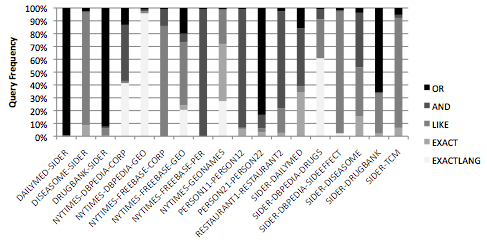
\includegraphics[height=90px ]{p8.png}
\caption{A naive attribute query over discriminative instances produces smaller candidates sets.} 
\end{figure} 

%An attribute query only produces empty sets if the threshold is to restrictive, the attribute alignment does not reflect the instances of data or if the matches do not exist.  In the other hand, it only produces high cardinality sets, when the threshold is too relaxed. We propose an initial algorithm to generate the attribute query that will be used as the heuristic. To define this attribute query, we have to define an alignment, a similarity measure and a threshold. On this attribute query (the heuristic), we fixed the similarity measure (we use the state of the art string based similarity measure) and the threshold that has a average performance related to this measure. Therefore, we focus in selecting the alignments that does not produce an empty set, i.e., we select only attribute pair that their values are similar w.r.t our similarity measure. To get these alignments, our elementary algorithm test all alignments for a significant sample of the instances and select the alignment that do not produce an empty set.

In that fashion, we expect to produce the minimum candidate set, with maximum recall. We need further improvements to the algorithm that select the queries, i.e.; we need to improve the algorithm that solve QSP.  The next section shows some preliminary results of this work so far.

